%%%%%%%%%%%%%%%%%%%%%%%%%%%%%%%%%%%%%%%%%%%%%%%%%%%%%%%%%%%%%%%%%%%%%%%%
% Plantilla TFG/TFM
% Escuela Politécnica Superior de la Universidad de Alicante
% Realizado por: Jose Manuel Requena Plens
% Contacto: info@jmrplens.com / Telegram:@jmrplens
%%%%%%%%%%%%%%%%%%%%%%%%%%%%%%%%%%%%%%%%%%%%%%%%%%%%%%%%%%%%%%%%%%%%%%%%

\chapter{Introducción}

\par A lo largo de este trabajo de final de grado se van hacer alusiones a parte de los conceptos básicos de Ingeniería de Telecomunicaciones que han sido impartidos durante el grado. Es por ello que en esta introducción se realizará un repaso de estos conceptos, términos y teorías imprescindibles para poder realizar y entender este estudio.
\\
\par Se realizará también una breve contextualización del proyecto para dar a entender la necesidad de esta tecnología de antenas para la nueva generaciones de comunicación movil en actual desarrollo: El 5G. 

\section{Las Telecomunicaciones}

\par Para entender el concepto de "Telecomunicación" es importante fijarse en cómo la etimología de la palabra nos lleva hasta su raíz: \textit{Comunicación}. La comunicación, en su significado más primitivo, es el proceso de intercambio de información entre dos sujetos definidos: Un emisor que genera y emite esta información, y un receptor que la recibe y la procesa. Además, en el proceso de comunicación siempre vamos a encontrar un tercer interviniente: El medio, encargado de transportar la información entre ambos sujetos. Por otro lado, nos queda el prefijo \textit{Tele}, proveniente del Griego: Lejos o Distancia. Se si regresa a la palabra original se puede definir el concepto de \textit{telecomunicación} como: El proceso de intercambio de información a distancia, y aunque es una definición correcta, dista del concepto de "Telecomunicaciones" que es utilizado día a día el cual, trae consigo la incursión de la tecnología en él. Es por ello que la Real Academia Española (RAE) define el concepto de \textit{telecomunicación} como:

\begin{quote}

\small Sistema de transmisión y recepción a distancia de señales de diversa naturaleza por medios electromagnéticos.

\end{quote}

\par En esta nueva definición incluimos un nuevo concepto imprescindible para poder adentrarnos a las telecomunicaciones actuales: El electromagnetismo o la interacción entre campos eléctricos y magnéticos. Este último concepto hace que se pueda entender actualmente a las telecomunicaciones como una rama científica que estudia la transmisión de información, no entre sujetos personales como se han entendido hasta ahora, sino entre máquinas. Cualquier máquina  ahora podrá actuar como un sujeto transmisor, que podrá emitir información codificada de una manera determinada de forma que uno o más receptores sean capaces de recibir, decodificar y procesar esta información de manera automática.
\\
\par El electromagnetismo es la rama de la ciencia encargada de estudiar la interacción entre partículas cargadas con campos eléctricos y magnéticos. El conjunto de fenómenos electromagnéticos que se conocen hoy en día fueron estudiados por científicos como \textit{H.C. Ørsted}, \textit{André-Marie Ampère}, \textit{Michael Faraday} y unificados por \textit{James Clerk Maxell} en su obra de 1865, \textit{A dynamical theory of the electromagnetic field}, donde se recogen las denominadas "Ecuaciones de Maxwell". La transmisión de la comunicación entre máquinas se realizará mediante impulsos eléctricos que, dada su naturaleza a variar con el tiempo y teniendo en cuenta esta teoría se transformaran en impulsos magnéticos y viceversa. Estos impulsos electromagnéticos se transmitirán a través de un medio, en forma de ondas electromagnéticas. A lo largo de los sigueintes capítulos se estudiará con más detenimiento los conceptos relacionados con las ondas y el medio.

\section{Teoría de señales}

\par Como se mencionó anteriormente, en el proceso de comunicación en el ámbito de las telecomunicaciones la información se envía en forma de señales. Se consideran las señales como un conjunto de impulsos electromagnéticos transmitidos por un emisor y codificados de una manera determinada para que el o los receptores a los que vaya dirigido puedan procesar la información contenida en una señal o conjunto de ellas. Esta información transmitida en forma de señales es el mensaje.
\\
\par Una señal electromagnética se caracteriza por el hecho de variar su intensidad en el dominio temporal. El ejemplo más básico lo encontramos en la onda Seno o Coseno de la figura
\ref{fig:seno}. De esta señal es posible obtener tres parámetros básicos imprescindibles para describir cualquier señal: Amplitud, frecuencia y fase. Se define la amplitud como la variación máxima respecto a un origen determinado y es medido en una magnitud física concreta, en el caso mencionado, la amplitud sería de una unidad, pudiendo ser esta voltios o vatios entre otros. Al tratarse de una señal oscilante aparece el concepto de frecuencia como el número de veces que la señal vuelve a su origen en un tiempo determinado de 1 segundo, la unidad de medida de este parámetro es el \textit{hertzio} (\textbf{Hz}), para el caso mencionado, la frecuencia de la onda es de 1 Hz, puesto que en un segundo la onda realiza un ciclo completo. Finalmente, se denomina fase al concepto de adelanto o retraso de la onda en el dominio temporal con respecto a un origen determinado, normalmente es representado mediante el símbolo \textit{phi} (\textbf{Φ}) y es medido en grados o radianes según sea conveniente, para el caso mencionado la fase sería 0º, puesto que se conoce que una onda sena tiene origen en este valor y no se aprecia ningún adelanto o retraso en la onda mencionada con respecto a este. Es posible agrupar estos parámetros en forma de ecuación analítica \ref{eq: seno} para el caso de una onda simple sin perdidas físicas ni amortiguación y con un movimiento armónico simple como:

\begin{equation}
	x(t)=A\cdot \sin(2\cdot\pi\cdot f+\phi )
	\label{eq: seno}
\end{equation}



\begin{figure}[h]
    \centering
        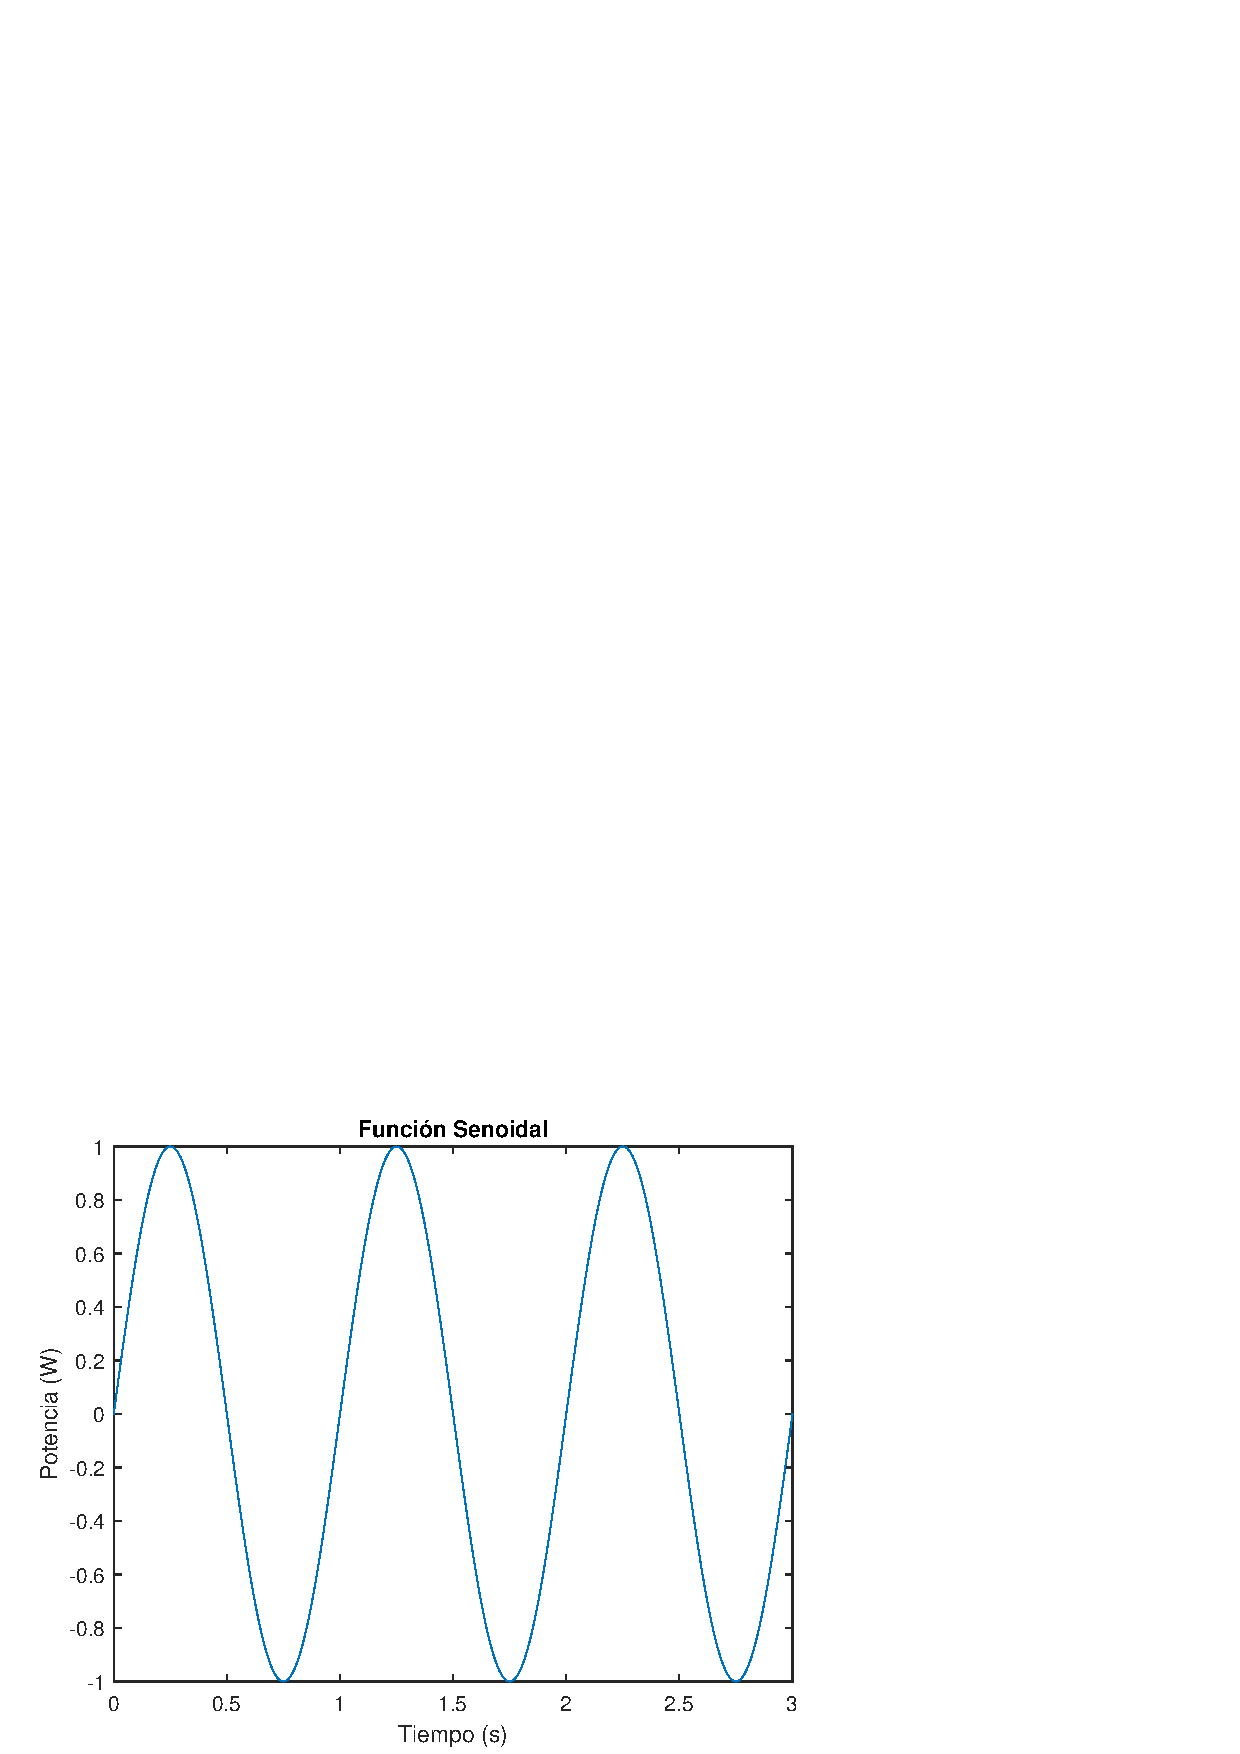
\includegraphics[width=15cm]{archivos/seno}
        \caption{Ejemplo de funcion senoidal}
        \label{fig:seno}
\end{figure}

\par A partir de los parámetros básicos de las ondas es posible el desarrollo de otros parámetros alternativos que facilitan su comprensión y análisis como son: La longitud de onda, definida como la distancia entre los picos o valles de una onda o el periodo, definido como el tiempo que tarda una onda en recorrer un ciclo completo. Estos dos nuevos parámetros se representan en las ecuaciones \ref{ecu:wavelength} y \ref{ecu:periodo} donde \textit{c} es la velocidad de la onda y \textit{f} la frecuencia de esta.

\begin{subequations}
	\begin{eqnarray}
		\lambda &=& \frac{c}{f} \label{ecu:wavelength} \\ % Salto de línea
		T &=& \frac{1}{f} \label{ecu:periodo}
	\end{eqnarray}
\end{subequations}

\par Pero ondas como la que se hacen referencia en la figura \ref{fig:seno}, cuyo tipo de movimiento: Movimiento armónico simple, no reflejan la realidad y la complejidad de las ondas reales que se usarán para la transmisión de información mediante ondas electromagnéticas. Otros conceptos como la atenuación o la amortiguación han de ser tomados en cuenta para describir con mayor precisión el comportamiento de las ondas en medios de transmisión reales como el aire. Si nos centramos en las \gls{oem}, encargadas de transportar los mensajes en forma de energía electromagnética, encontramos que el medio en el que se propagan, no tiene /todo{porque por qué} ser necesariamente el aire, ya que estas se pueden propagar en el vacío. En este medio, las \gls{oem} se propagarán a una velocidad de 300 000 000 m/s, o más conocida como la velocidad de la luz, ya que la luz en sí es una onda electromagnética. 
\\
\par Cuando analizamos un conjunto de partículas subatómicas (electrones o protones) se puede comprobar como a sus alrededores se producen campos eléctricos debido a la interacción entre estos, de repulsión o atracción. A su vez, el hecho de provocar esta interacción en forma de movimiento de las partículas, se producirá un campo magnético sobre estas. Es entonces donde, la suma de ambos campos debido a las interacciones entre partículas producen campos electromagnéticos, medio donde se propagaran las \gls{oem}.
\\
\par Las \gls{oem} se pueden caracterizar como cualquier otra onda, por la ecuación de ondas \ref{ecu:onda}
\begin{equation}
	\nabla^2\psi(\vec r, t)=\dfrac
1{v^2}\dfrac{\partial^2\psi
(\vec r,t)}{\partial t^2}
	\label{eq: onda}
\end{equation}


\par Hasta el momento solo se ha mencionado las señales como mensajes codificados en ondas electromagnéticas que varían en el dominio temporal, pero gracias al matemático Joseph Fourier (1768 - 1830), se pudo empezar a estudiar las ondas desde otro dominio: La frecuencia. Fourier desarrolló una serie de transformaciones matemáticas capaces de convertir las expresiones analíticas descritas en un dominio temporal a un dominio frecuencial y viceversa, a las que denominó: \textit{Transformada de Fourier}, basadas en el \textit{Teorema de Fourier} el cual señala que cualquier señal periódica puede descomponerse mediante una suma infinita de funciones de tipo sinusoidal ponderadas de forma determinada en amplitud y fase y cuyas frecuencias estén relacionadas armónicamente con la frecuencia fundamental de la onda a analizar. 
\\
\par Gracias a la Transformada de Fourier podemos analizar y sintetizar cualquier onda independientemente de su naturaleza física o matemática, y aunque no será usada como tal a lo largo de este trabajo, se hace necesario remarcar la importancia de este desarrollo matemático y la imprescindible contribución hacia el desarrollo de áreas como la acústica o las telecomunicaciones ya que todo avance realizado en esta materia tiene intrínseca la participación de la Transformada de Fourier, como es en nuestro caso, en el que toda representación de señales se realizará en el dominio frecuencial. 

\section{5G}

\par El \gls{5g} es el nuevo estandar de telefonía móvil, sucesora de la \gls{4g}, llevado a cabo por el \gls{3gpp} en su Release 15 y 16. Este nuevo estandar de telefonía permitirá:
\begin{itemize}
\item Conexiones con throughputs, o tasas de rendimiento efectivas de hasta 10 Gbps, es decir, hasta 10 veces más rapido que el \gls{4g}.
\item La latencia, definida como la suma de retrasos temporales producidas en un sistema de comunicación debido a la velocidad de propagación limitada, perdidas, etc. se reducirán hasta valores de 1 ms en comparación con el rango de entre 30 y 50 ms que obtenemos en redes \gls{4g} y \gls{wifi}
\item Capacidad de conexiones masivas para dispositivos \gls{iot} lo que permitirá  el desarrollo de redes de comunicación \gls{m2m} aumentando la eficiencia energética de estas, así como su disponibilidad y seguridad, lo que será imprescindible para tecnologías emergentes como la conducción autónoma o las Smart Cities, es decir, el proceso de uso de las \gls{tic} para modernizar el entorno urbano ofreciendo servicios de mejora del transporte público, seguridad ciudadana, ahorro energético, etc.
\item Mejora de la diversidad en recepción con respecto al \gls{4g} mediante el uso del \gls{mimo} Masivo. Esta tecnología aprovecha el uso de múltiples antenas sobre un mismo dispositivo para usarlas como enlaces independientes, de forma que la velocidad de conexión pueda aumentar de forma significativa. Con \gls{mmimo} se dispondrán de decenas de antenas por dispositivo para hacer que la conexión sea más rápida y eficiente.
\item El uso del beamforming, proceso por el cual se direcciona el haz de emisión de la antena y mediante técnicas de procesado digital se calcula en qué dirección se hará más eficiente la comunicación entre la antena y el dispositivo además de poder hacer cálculos sobre ruido e interferencias para mejorar la eficiencia de la antena.
\end{itemize}

\par Además, el \gls{5g} emitirá sobre nuevas bandas de frecuencia, las cuales categorizaremos como \textit{Bandas Sub-6Ghz} y \textit{Bandas Super-6Ghz}. En el caso del plan nacional para el 5G aprobado por el \gls{minetur}, principal responsable de la gestión de los temas referentes a telecomunicaciones a nivel estatal en España, las bandas de frecuencias aprobadas para el 5G son:
\begin{itemize}
\item\textbf{700 Mhz:} Esta banda antes usada para la retransmisión de la \gls{tdt} y adjudicada para su uso en el \gls{5g} mediante el segundo dividendo digital será clave para la retransmisión de señales móviles \gls{5g} que necesitan alcanzar los interiores de los hogares y las oficinas puesto que su mayor longitud de onda con respecto a otras bandas la hace apta para penetrar o difractar sobre muros.
\item\textbf{3.4-3.8 Ghz: }Estas bandas de frecuencias eran anteriormente usadas para radioenlaces de transporte de señal de televisión, actualmente en desuso. Permitirán mayores tasas de velocidad con respecto a los 700 Mhz, pero su atenuación será mayor, lo que la hace adecuada para transmisión en zonas urbanas o carreteras.
\item\textbf{26 Ghz: }En este rango de frecuencias entramos en las denominadas como \gls{mmwv} es decir, ondas cuya longitud de onda esté en el orden de milímetros. Esta banda de frecuencia presume de tener mayor disponibilidad en cuanto a ancho de banda lo que permitirá conexiones de banda ancha ultrarápidas.
\end{itemize}

\par Como se puede, la tendencia futura en cuanto a comunicaciones móviles de alta velocidad va de la mano y es directamente proporcional a la frecuencia a la que se emita la señal, pero a su vez, este incremento de frecuencia hace más vulnerables a las transmisiones de ser interferidas o atenuadas durante su retransmisión, lo que haría muy difícil el uso de las redes \gls{5g} cuando la antena se sitúa en el exterior y los dispositivos en interiores. En este escenario surge el concepto, ya existente en el \gls{4g} del uso de Small Cells. Las Small Cells son pequeñas estaciones base que se sitúan en puntos estratégicos tanto en interiores como oficinas o centros comerciales, como en exteriores en sitios con una gran afluencia de personas y por ende, de dispositivos móviles. 
\\
\par En el \gls{5g}, el concepto de Small Cell es imprescindible. Debido al crecimiento exponencial del uso de dispositivos por parte de usuarios y empresas cada vez se hará más difícil el hecho de que una sola estación base pueda dar cobertura y una tasa de transmisión aceptables al estándar a estos dispositivos. Es por ello que en los nuevos despliegues de \gls{5g} las operadoras se inclinarán más por el uso de muchas Small Cells a lo largo de la ciudad que den servicio a los usuarios de un rango muy limitado de espacio, pero con muy buena cobertura y tasas de transmisión, que a la instalación de estaciones base convencionales que dan cobertura en radios muy amplios de distancia, lo que en grandes urbes puede suponer la saturación de la propia estación base.
\\
\par Bajo todo este nuevo escenario de comunicaciones avanzadas que plantea para un futuro muy cercano se han de plantear qué tecnologías se usarán para cubrir las metas y especificaciones marcadas de la manera más robusta y eficiente. El \gls{5g} tendrá una completa dependencia de los sistemas informáticos diseñados para alcanzar estas metas, mediante técnicas de procesado digital y nuevos algoritmos podremos ir añadiendo características e incluso mejorando las ya existentes sin necesidad de alterar todo el sistema ya instalado en la red. Pero no se ha de olvidar cuáles son los elementos básicos de comunicación: Los sujetos y el medio.

\section{Motivación}

\par Como hemos mencionado en la sección \todo{Mencionar secciones} 1.1, la comunicación se realiza a través de un medio y este puede tener dos naturalezas: Guiado o radiado. El medio guiado o alámbrico es aquel que depende de una superficie conductora para transmitir la información, por lo general, un cable con propiedades conductoras como cobre u oro, pero también entran en esta categoría la fibra óptica, que transmite por sus filamentos los mensajes codificados en impulsos de luz.  
\\
\par Por otro lado tenemos el medio radiado o también denominado inalámbrico o no guiado, cuyo medio de transporte son los campos electromagnéticos. En este medio no es posible observar las ondas viajar por el espacio, exceptuando el rango de frecuencias correspondiente a la luz visible dentro del espectro electromagnético. Una de las principales propiedades de este medio es que las ondas que viajan a distinta frecuencia son inmunes entre sí a interferirse, lo que permite que los mensajes lleguen del emisor al receptor sin apenas haber sido afectadas en su trayecto por otros mensajes viajando por el campo electromagnético. A partir de ahora el papel del emisor y receptor será tomado por las antenas, las cuales serán capaces de enviar o recibir señales transmitidas en el campo electromagnético en una o varias frecuencias o longitudes de onda. Es por esto que las antenas quedan ahora como los elementos claves para la transmisión de información inalámbrica. 
\\ 
\par En la actualidad existen varios tipos de antena, como estudiaremos más detenidamente en el \todo {tema 3?} y cada uno de ellas se adaptará más específicamente a nuestras necesidades de directividad, ganancia, ancho de banda o eficiencia entre otros. En el estudio que nos ocupa, se diseñará un array de parches en tecnología microstrip que será capaz de trabajar a las frecuencias especificadas para la \gls{5g} de comunicaciones móviles por el \gls{3gpp}.

\section{Estructura del proyecto y metodología}

\par Este proyecto estará dividido en dos partes fundamentales, un marco teórico, donde se realizará una completo marco teórico sobre los conceptos básicos de las líneas de transmisión: Adaptación e impedancias, tecnología microstrip en líneas de transmisión, etc. Antenas: Tipos de antena, parámetros de estudio básicos, etc. Y en un marco más específico, sobre las antenas de tipo parche en tecnología microstrip: Métodos de alimentación, componentes, tipos, análisis, etc. Finalmente se expondrá la parte de experimentación, donde se estudiarán y analizarán los diseños de distintos tipos de configuraciones de arrays para antenas de tipo parche con tecnología microstrip.
\\
\par Para realizar la parte experimental del proyecto se hará uso del software de análisis electromagnético 3D: Ansys\sffamily\textregistered  HFSS (High Frequency Structure Simulator). Este software es usado para diseñar y simular componentes electrónicos de alta frecuencia como antenas, arrays, filtros o placas de circuito impreso. Con el, se diseñarán las configuraciones de antenas especificadas y se simularan sus efectos electromagnéticos como si se tratara de una cámara anecóica, para finalmente poder analizar los resultados obtenidos y los valores de los parámetros característicos de la antena así como comprobar la viabilidad del producto final en términos de rendimiento o dimensiones.
\\
\par Por otro lado, se hará uso de la herramienta de cálculo matemático MathWorks\sffamily\textregistered  MATLAB, con la que realizaremos cálculos básicos sobre las dimensiones de la antena a diseñar en función a los parámetros de construcción de esta.
